\documentclass[12pt,modern,tighten,times,apj]{aastex61}

\newcommand{\sigv}{{\ensuremath{\langle \sigma v \rangle}}}
\newcommand{\eg}{e.g.}
\newcommand{\alp}{\ensuremath{\alpha}}
\newcommand{\thsp}{\thinspace}
\newcommand{\cc}{\ensuremath {\mathrm{cm^{3}}}}
\newcommand{\gcc}{\ensuremath{\mathrm{\thsp g \thsp cm^{-3}}}}
\newcommand{\kel}{\ensuremath{\mathrm{\thsp K}}}
\newcommand{\gk}{\ensuremath{\mathrm{\thsp GK}}}
\newcommand{\calN}{\ensuremath {\mathcal N}}
\newcommand{\calZ} {\ensuremath {\mathcal {Z}}}
\newcommand{\isotope}[2]{\ensuremath{\mathrm{^{#2}#1}}}
\newcommand{\ye}{\ensuremath{Y_{e}}}


\begin{document}

\title{XNet}

\section{Introduction}

Represented numerically as a system of first order differential equations, the nuclear reaction network has sink and source terms representing each of the many nuclear reactions involved. 
XNet is group of routines, written in FORTRAN95, designed to solve arbitrary nuclear reaction networks of astrophysical interest. 
To explain the functionality of XNet, we begin by briefly outlining the sets of reactions we must solve to evolve the nuclear composition.  
To this end, we present a brief overview of the thermonuclear reaction rates of interest and how these rates are assembled into the differential equations that must ultimately be solved.
For more detailed information, we refer the reader to several textbooks covering this subjects \cite{Clay83,RoRo88,Arne96}.  
We follow this with a discussion of the solvers included within XNet.
Because the rate equations in nucleosynthetic applications involve a wide range of timescales, implicit methods have proven mandatory, leading to the need to solve matrix equations. 
Efforts to improve the performance of such rate equation methods are focused on efficient solution of these matrix equations, in particular by making best use of the sparseness of these matrices, and finding methods that require less frequent matrix solutions.  

\section{Reaction Rates}\label{sect:reacrate}

There are a large number of types of nuclear reactions which are of astrophysical interest, most of which are included in XNet.  
In addition to the emission or absorption of  nuclei and nucleons, nuclear reactions can involve the emission or  absorption of photons ($\gamma$-rays) and leptons (electrons, neutrinos,  and their anti-particles).  
As a result, nuclear reactions involve three of the  four fundamental forces, the nuclear strong, electromagnetic and nuclear weak forces.  
Reactions involving leptons (termed weak interactions) proceed  much more slowly than those involving only nucleons and photons;  however,  these reactions are important because only weak interactions can change the global ratio of protons to neutrons.

The most basic piece of information about any nuclear reaction is the nuclear cross section.  
The cross section for a reaction between target $j$ and projectile $k$ is defined by 
\begin{equation}
    \sigma = {\rm{number\ of\ reactions\ target^{-1} sec^{-1}} \over
    {flux\ of\ incoming\ projectiles}} = {{r/n_j} \over {n_k v}}. 
    \label{eq:sigma}
\end{equation}
The second equality holds when the relative velocity between targets of number density $n_j$ and projectiles of number density $n_k$ is constant and has the value $v$.  
Then $r$, the number of reactions per $cm^{-3}$\ and sec, can be expressed as $r=\sigma v n_j n_k$.  
More generally, the targets and projectiles have distributions of velocities, in which case $r$ is given by
\begin{equation}
    r_{j,k}=\int \sigma (\vert \vec v_j -\vec v_k\vert) \vert \vec v_j 
    -\vec v_k\vert d^3 n_j d^3 n_k.
    \label{eq:rate}
\end{equation}
The evaluation of this integral depends on the types of particles and distributions which are involved. For nuclei $j$ and $k$ in an astrophysical plasma, Maxwell-Boltzmann statistics generally apply; thus,
\begin{equation}
    d^3n=n ({{m} \over {2\pi k_B T}})^{3/2} \exp (-{{mv^2} \over {2 k_B T}}) d^3v,
\end{equation}
allowing $n_j$ and $n_k$ to be moved outside of the integral.  
Eq.~\ref{eq:rate} can then be written as $r_{j,k}=\sigv_{j,k} n_j n_k$, where \sigv\ is the velocity integrated cross section.  
Equivalently, one can express the reaction rate in terms of a mean lifetime of particle $j$ against destruction by particle $k$, 
\begin{equation}
    \tau_{k}(j)= {1 \over {\sigv_{j,k} n_{k}}}
    \label{eq:tau}
\end{equation}

For thermonuclear reactions, these integrated cross sections have the form \cite{Clay83,FoCZ67}
\begin{equation}
    \langle j,k \rangle \equiv \sigv_{j,k}= ({8 \over {\mu \pi}})^{1/2} 
    (k_B T)^{-3/2} \int_0 ^\infty E \sigma (E) {\rm exp}(-E/k_B T) dE, 
    \label{eq:sigv}
\end{equation}
where $\mu$ denotes the reduced mass of the target-projectile system, $E$ the center of mass energy, $T$ the temperature and $k_{B}$ is Boltzmann's constant.

Experimental measurements and theoretical predictions for these reaction rates provide the data input necessary to study astrophysical thermonuclear kinetics.  
While detailed discussion of individual rates is beyond the scope of this article, the interested reader is directed to the following reviews, in this volume and elsewhere.  
Experimental nuclear rates and the methodology for measuring them have been reviewed in detail by \cite{RoRo88,KaTW98}.  
A number of articles in this volume review the charged particle reaction rates which are important in the Sun \cite{HaPR04}, in later stages of stellar evolution \cite{BuBa04}, and for explosive burning on compact objects \cite{AnSB04,HeJI04,ReSc04}.  
Experimental neutron capture cross sections are also summarized \cite{KaMe04,BaKa00}.  
Theoretical modeling of these rates \cite{RaDe04,MaNW04} is vitally important to provide the many rates for which experimental information is incomplete or non-existant.  
Beyond measuring or calculating these rates, progress in nuclear astrophysics also requires the compilation and dissemination (in a usable form) of this hard-earned nuclear data to the broadest astrophysical community \cite{CaFo88,GRSD04,Smit03}. 

When particle $k$ in Eq.~\ref{eq:rate} is a photon, the distribution $d^3n_k$ is given by the Plank distribution,  
\begin{equation}
    d^3n_{\gamma} =  {{8 \pi} \over {c^3 h^3}} {{E_{\gamma}^2} \over
    {\exp \left(E_{\gamma} /k_B T\right)-1}} dE_{\gamma} \ .
\end{equation}
Furthermore, the relative velocity is always $c$ and thus the integral is separable, simplifying to 
\begin{equation}
    r_j  = {{\int d^3n_j}\over {\pi ^2 (c \hbar )^3}} \int_0 ^\infty {{c 
    \sigma(E_\gamma ) E_{\gamma}^2} \over {{\rm exp}(E_\gamma /k_B T) -1}} dE_
    \gamma \equiv \lambda_{j,\gamma} (T) n_j. 
    \label{eq:phrate}
\end{equation}
In practice it is not usually necessary to directly evaluate the photodisintegration cross sections (see, however, \cite{MoZU04} for exceptions), because they can be expressed by detailed balance in terms of the capture cross sections for the inverse reaction, $l+m\rightarrow j+\gamma$ \cite{FoCZ67} .
\begin{equation}
    \lambda_{j,\gamma} (T)= ({{G_l G_m} \over G_j}) ({{A_l A_m} \over A_j})
    ^{3/2} ({{m_u k_B T} \over {2\pi \hbar^2}})^{3/2} \langle l,m \rangle 
    \exp (-Q_{lm}/k_B T).
    \label{eq:detbal}
\end{equation}
This expression depends on the partition functions, $G_{k}=\sum_i (2J_i+1) \exp (-E_i/k_B T)$ (which account for the populations of the excited states of the nucleus), the mass numbers, $A$, the temperature $T$, the inverse reaction rate $\langle l,m \rangle$, and the reaction $Q$-value (the energy released by the reaction), $Q_{lm}=(m_l+m_m-m_j) c^2$.  
Since photodisintegrations are endoergic, their rates are vanishingly small until sufficient photons exist in the high energy tail of the Planck distribution with energies $> Q_{{lm}}$.  
As a rule of thumb this requires $T$$\approx$$Q_{lm}/30 k_{B}$.

In practice, these experimental and theoretical reaction rates are determined for bare nuclei, while in astrophysical plasmas, these reactions occur among a background of other nuclei and electrons.  
As a result of this background, the reacting nuclei experience a Coulomb repulsion modified from 
that of bare nuclei. 
For high densities and/or low temperatures, the effects of this screening of reactions becomes very important. 
Under most conditions (with non-vanishing temperatures) the generalized reaction rate integral can be separated into the traditional expression without screening [Eq.~\ref{eq:sigv}] and a screening factor, 
\begin{equation}
    \langle j,k \rangle^*=f_{scr}(Z_j,Z_k,\rho,T,n_i) \langle j,k \rangle. 
    \label{eq:screen}
\end{equation}
This screening factor is dependent on the charge of the involved particles, the density, temperature, and the composition of the plasma. For more details on the form of $f_{scr}$, see, \eg, \cite{Salp54,DeGC73,Ichi93,BrSa97}.  
At high densities and low temperatures screening factors can enhance reactions by many orders of magnitude and lead to {\em pycnonuclear ignition}.
In the extreme case of very low temperatures, where reactions are only possible via ground state oscillations of the nuclei in a Coulomb lattice, Eq.~\ref{eq:screen} breaks down, because it was derived under the assumption of a Boltzmann distribution \cite{SaVa69,IcKi99}.

In stellar plasmas, target nuclei also do not exist solely in their ground states.  
This complicates the rate expression in Eq.~\ref{eq:sigv}, which now must take into account the cross sections for capture out of the different excited states and properly weight them according to their probability of occurrence in the ensemble of target nuclei.  
Because the timescales for transitions between excited states of a nucleus are typically much shorter than other reaction timescales, it is usually valid to assume that the nuclei are internally equilibrated and a given excited state is populated in the ensemble by the usual Boltzmann factor $\propto e^{-E/k_BT}$, where $E$ now is the excitation energy of that state.  
From this, one may derive a factor, called the {\em stellar enhancement factor} (SEF), to correct the ground-state reaction rate for the population of excited states (see, e.g., \cite{RaTh00,AARD99}).

Interesting complications to this prescription arise when the internal
equilibration timescale for a nucleus exceeds the other reaction
timescales in the problem.  This usually occurs when a large spin
difference between the ground state of an isotope and its first excited state
prevents them from communicating directly via internal transitions.
The isotope $^{26}$Al is the prototypical example, with a ground and isomeric state of spin and parity $5^+$ and $0^+$, respectively.  When these two states equilibrate, it is not through a direct transition between the states--that simply takes too long.  Rather the equilibration occurs
through transitions to higher-lying levels that communicate effectively
with both levels.  This problem has been studied in detail (e.g.,
\cite{WaFo80}), and the most straightforward way of dealing with this is
to assume that the higher-lying levels are in a steady state since their
destruction timescales are so rapid.  When this is done, the population of
the target nucleus break up into two ensembles, one tied to the ground
state and one tied to the isomer \cite{GuMe01}.  These may then be treated
as separate species in the network, each with its own rates to and from
other isotopes and with effective rates for transitions between the two
ensembles.  Fortunately, the number of nuclei requiring such treatment is
small and does not add much computational burden to running the nuclear
reaction network.

A procedure similar to that used to derive Eq.~\ref{eq:phrate} applies to captures of electrons by nuclei.  Because the electron is 1836 times less massive than a 
nucleon, the velocity of the nucleus $j$ in the center of mass system is 
negligible in comparison to the electron velocity ($\vert \vec v_j- \vec 
v_e \vert \approx \vert \vec v_e \vert$).  In the neutral, completely 
ionized plasmas typical of the astrophysical sites of nucleosynthesis, the 
electron number density, $n_{e}$, is equal to the total density of protons 
in nuclei, $\sum_i Z_i n_i$.  However in many of these astrophysical 
settings the electrons are at least partially degenerate, therefore the 
electron distribution cannot be assumed to be Maxwellian.  Instead the 
capture cross section may be integrated over a Boltzmann, partially 
degenerate, or degenerate Fermi distribution of electrons, depending on the 
astrophysical conditions.  The resulting electron capture rates are 
functions of $T$ and $n_e$, $r_j=\lambda_{j,e} (T,n_e) n_j.$  Similar equations apply for the capture of positrons which are in thermal equilibrium with photons, electrons, and nuclei.  Electron and positron capture calculations have been performed for a large variety of nuclei with mass numbers between A=20 and A=100 (see \cite{LiMF04} for more information). 
For normal decays, like beta or alpha decays, with a characteristic  half-life
$\tau_{1/2}$,  Eq.~\ref{eq:phrate} also applies, with the
decay constant  $\lambda_j=\ln 2/\tau_{1/2}$.  In addition to innumerable
experimental half-life determinations, beta-decay half-lives for a wide range of unstable nuclei have  been predicted (see \cite{Borz04,MoNK97}).

Even though the size of the neutrino scattering cross section on nuclei and electrons is very small, at high densities ($\rho \sim 10^{13} \gcc$), enough scattering events occur to thermalize the neutrino distribution.  Under such conditions the inverse process to electron capture (neutrino capture) can occur in significant numbers and the neutrino capture rate can be expressed in a form similar to Eqs.~\ref{eq:phrate} by integrating over the thermal 
neutrino distribution (e.g. \cite{FuMe95}).  Inelastic neutrino scattering 
on nuclei can also be expressed in this form.  The latter can cause 
particle emission, similar to photodisintegration.  See \cite{BuRe04,Brue85,Voge04} for more complete discussion of the interactions of neutrinos with matter.  The calculation of these rates 
can be further complicated by the neutrinos being out of thermal 
equilibrium with the local environment.  When thermal equilibrium among 
neutrinos was established at a different location, then the neutrino 
distribution might be characterized by a chemical potential and a 
temperature different from the local values.  Otherwise, the neutrino 
distribution must be evolved in detail (see, \eg, \cite{MeMe99}). 

\subsection{Screening}

While much of the literature on the screening of nuclear reactions has focused on the screening of fusion reactions, this same physics is important when reaction pairs have equilibrated, be it local quasi-equilibrium (QSE) or global Nuclear Statistical Equilibrium (NSE) \citep{HiTh96,BrGa99}.
If equilibrium abundances calculated from thermonuclear reaction networks using these fusion rates are to match the abundances calculated from equilibrium expressions, the relevant screening factors must be calculated consistently.
Using the velocity integrated cross section $\langle \sigma v \rangle$, the screened cross section for the reaction of nuclei $i$ and $j$ is defined in terms of the unscreened cross section by
\begin{equation}
{\langle \sigma v \rangle}_{screened\ nuclei} = \exp(H_{ij}) {\langle 
\sigma v \rangle}_{bare\ nuclei} \ ,
\end{equation}
where $\exp(H_{ij})$ is termed the screening enhancement factor, sometimes denoted $f_{scr}$.
 
Screening enters the equilibrium expressions for NSE or QSE as a modification of the nuclear binding energy, $H(Z)$, that is the difference in the Helmholtz free energy due to screening in assembling the nucleus $^AZ$.
Some screening laws, like Salpeter's original weak and strong screening laws \citep{Salp54}, are derived analytically from this same change in the free energy \citep[see also][]{DeGrCo73}.  
Given an expression for the change in free energy $H(Z)$, the screening factor for reaction rates can be computed from 
\begin{equation}
H_{ij} = (H(Z_i+Z_j)-H(Z_i)-H(Z_j))/k_B T.
\end{equation} 
Other screening laws are the product of fits to Monte Carlo plasma simulations \citep[see, for example,]{OgIyIc91}
Within statistical uncertainties, these alternative methods produce consistent results \citep[see, for example,][]{DeSl99,Rose92}.

Previously, \citet{HiTh96} had constructed the NSE screening term sequentially from $H_{p,\gamma}$ terms to maintain consistency with the nuclear reaction network results, whereas \citet{BrGa99} computed NSE screening terms from global Coulomb corrections using various moments in powers of $Z$ over the NSE abundance distribution.  
Where $H_{p,\gamma} = (H(Z+1)-H(Z)-H(1))/k_B T$, these results should be consistent. (Note $H(1)=0$, there is no reaction that builds a proton.)  

The necessity of this functional form for screening comes from the requirement that the change in the difference in the binding energy due to screening between two species must be independent of the reaction pathway.  
For example, the abundances of $^AZ$ and $^{(A+4)}(Z+2)$ can be kept in equilibrium by $(\alpha,\gamma)$ and it reverse or by the series $(p,\gamma) (p,\gamma) (n,\gamma) (n,\gamma)$ and their reverses. 
When constructed from $H(Z)$, this is requirement is manifestly met, $\Delta BE = H(Z+2)-H(Z)$.
Without this, you can not define a unique relation for the equilibrium screening correction that covers all of the reaction paths that are simultaneously in equilibrium between $^AZ$ and $^{(A+4)}(Z+2)$.
Further note that because the reaction pathways $(p,\gamma) (p,\gamma) (n,\gamma) (n,\gamma)$ and $(p,\gamma) (n,\gamma) (p,\gamma) (n,\gamma)$ are simultaneously in equilibrium, H(Z) can not depend on A.
%for example, $H_{\alpha,\gamma}$ = $H_{p,\gamma} + H_{p,\gamma} + H_{n,\gamma} + H_{n,\gamma} = H_{p,\gamma} + H_{n,\gamma} + H_{p,\gamma} + H_{n,\gamma}$, etc. 

For three reactant reactions, the screening factor for reaction rates is conventionally calculated as $H_{ijk} = H_{ij} + H_{(i+j)k}$ because three particle reactions of importance in astrophysics are generally sequential pairs of reactions where a short-lived intermediate nucleus $(i+j)$ is formed by the first pair of reactants and captures the third reactant before it decays.
To remain consistent with the requirements of equilibrium screening, we must construct $H_{ijk}$ from $H$.
In general, this approach should work as well for astrophysical 3 reactant reactions as for 2.  
\begin{eqnarray}
H(Z_i+Z_j+Z_k) &-&H(Z_i) - H(Z_j) - H(Z_k) \\
&=& \left(H(Z_i+Z_j+Z_k) - H(Z_i+Z_j) - H(Z_k)\right) \\
&+& \left(H(Z_i+Z_j) - H(Z_i) - H(Z_j)\right) \\
&=& H_{(i+j)k} + H_{ij} \\
&=& H_{ijk} \ . 
\end{eqnarray}
Thus the screening factors of 3 reactant reactions can be adequately calculated from the change in free energy. 

\subsubsection{Weak Screening}

For weak screening,  Graboske, Dewitt, Grossman \& Cooper (1973; ApJ 181 457), give $H_{12}$ in terms of charge independent parameter $\Lambda_0$, an average charge parameter $\tilde z$ which depends on the abundances of all nuclear species, and the ion charges $Z_i$ and $Z_j$ as 
\begin{equation}
H_{ij} = Z_i Z_j \tilde{z} \Lambda_0.  
\end{equation} 
$\Lambda_0$ and  $\tilde z$ are defined in \citet{DeGrCo73}. 
This expression approaches the classical Debye-H\"uckel case as the electrons become non-degenerate.  
Choosing the corresponding 
\begin{equation}
H(Z) = {1\over2} Z^2 \tilde{z} \Lambda_0 \ ,
\end{equation} 
then 
\begin{equation}
H(Z_i+Z_j) - H(Z_i) - H(Z_j) = {1\over2}\left((Z_i+Z_j)^2 - Z_i^2 - Z_j^2\right) \tilde{z} \Lambda_0  =  Z_i Z_j \tilde{z} \Lambda_0 = H_{ij}
\end{equation} 
Thus the equivalence of the approaches does indeed hold for two-reactant reactions.  
For three-reactant reactions, 
\begin{equation}
H_{ijk} = H_{ij} + H_{(i+j)k} = Z_i Z_j \tilde{z} \Lambda_0 + (Z_i+Z_j) Z_k \tilde{z} \Lambda_0 = (Z_i Z_j + Z_i Z_k + Z_j Z_k) \tilde{z} \Lambda_0 \ .
\end{equation}
In terms of H(Z)
\begin{eqnarray}
H(Z_i+Z_j+Z_k) &-&H(Z_i) - H(Z_j) - H(Z_k) \\
&=&  {1\over2}\left((Z_i+Z_j+Z_k)^2 - Z_i^2 - Z_j^2- Z_k^2\right) \tilde{z} \Lambda_0 \\
&=& (Z_i Z_j + Z_i Z_k + Z_j Z_k) \tilde{z} \Lambda_0 = H_{ijk} \ ,  
\end{eqnarray}
thus the equivalence of the approaches also holds for three-reactant reactions.  

\subsubsection{Intermediate Screening}

For intermediate screening,  \citet{DeGrCo73} give $H_{12}$ in terms of charge independent parameter $\Lambda_0$, and several average charge parameters $\tilde z$, $\bar z$, and $\langle z^{1.58}\rangle$, which depends on the abundances of all nuclear species, and the ion charges $Z_i$ and $Z_j$ as 
\begin{equation}
H_{ij} = 0.380 {\langle z^{1.58}\rangle \over \tilde{z}^{0.58}\bar{z}^{0.28}} \Lambda_0^{0.860} \left[(Z_i + Z_j)^{1.860} - Z_i^{1.860} - Z_j^{1.860}\right].  
\end{equation} 
Choosing the corresponding 
\begin{equation}H(Z) = 0.380 {\langle z^{1.58}\rangle \over \tilde{z}^{0.58}\bar{z}^{0.28}} \Lambda_0^{0.860} Z^{1.860}, \end{equation} then 
\begin{eqnarray}
H(Z_i+Z_j) &-& H(Z_i) - H(Z_j) \\
&=& 0.380 {\langle z^{1.58}\rangle \over \tilde{z}^{0.58}\bar{z}^{0.28}} \Lambda_0^{0.860} \left[(Z_i + Z_j)^{1.860} - Z_i^{1.860} - Z_j^{1.860}\right]= H_{ij}
\end{eqnarray} 
Thus the equivalence of the approaches does indeed hold for two-reactant reactions.  
For three-reactant reactions, 
\begin{eqnarray}
H_{ijk} &=& H_{ij} + H_{(i+j)k} \\
&=& 0.380 {\langle z^{1.58}\rangle \over \tilde{z}^{0.58}\bar{z}^{0.28}} \Lambda_0^{0.860} \left[(Z_i + Z_j)^{1.860} - Z_i^{1.860} - Z_j^{1.860}\right] \\
&+& 0.380 {\langle z^{1.58}\rangle \over \tilde{z}^{0.58}\bar{z}^{0.28}} \Lambda_0^{0.860} \left[(Z_i + Z_j+Z_k)^{1.860} - (Z_i + Z_j)^{1.860} - Z_k^{1.860}\right] \\
&=&  0.380 {\langle z^{1.58}\rangle \over \tilde{z}^{0.58}\bar{z}^{0.28}} \Lambda_0^{0.860} \left[(Z_i + Z_j+Z_k)^{1.860} - Z_i^{1.860} - Z_j^{1.860} - Z_k^{1.860} \right]
\ .
\end{eqnarray}
In terms of H(Z)
\begin{eqnarray}
H(Z_i+Z_j+Z_k) &-& H(Z_i) - H(Z_j) - H(Z_k) \\
&=&  0.380 {\langle z^{1.58}\rangle \over \tilde{z}^{0.58}\bar{z}^{0.28}} \Lambda_0^{0.860} \left[(Z_i + Z_j+Z_k)^{1.860} - Z_i^{1.860} - Z_j^{1.860} - Z_k^{1.860} \right]\\
&=&  H_{ijk} \ ,  
\end{eqnarray}
thus the equivalence of the approaches also holds for three-reactant reactions.

\subsubsection{Strong Screening}  



\section{Solvers}

The large number of reaction types discussed in \S \ref{sect:reacrate} can 
be divided into 3 functional categories based on the number of reactants 
which are nuclei.  The reactions involving a single nucleus, which include 
decays, electron and positron captures, photodisintegrations, and neutrino 
induced reactions, depend on the number density of only the target species.  
For reaction involving two nuclei, the reaction rate depends on the number 
densities of both target and projectile nuclei.  There are also a few 
important three-particle process (like the triple-\alp\ process, see \S \ref{sect:hyb}) which are commonly successive captures with an 
intermediate unstable target (see, \eg, \cite{NoTM85,GoWT95}).  Using an 
equilibrium abundance for the unstable intermediate, the contributions of 
these reactions are commonly written in the form of a three-particle 
processes, depending on a trio of number densities.  Grouping reactions by 
these 3 functional categories, the time derivatives of the number densities 
of each nuclear species in an astrophysical plasma can be written in terms 
of the reaction rates, $r$, as
\begin{equation}
    \left. {{\partial n_i} \over {\partial t}} \right|_{\rho =const}= \sum_j 
    \calN^i _j r_j + \sum_{j,k} \calN^i _{j,k} r_{j,k} + \sum_{j,k,l} 
    \calN^i _{j,k,l} r_{j,k,l},
    \label{eq:ndot}
\end{equation}
where the three sums are over reactions which produce or destroy a nucleus 
of species $i$ with 1, 2 \& 3 reactant nuclei, respectively.  The \calN\ s
provide for proper accounting of numbers of nuclei and are given by: 
$\calN^i_j = N_i$, $\calN^i_{j,k} = N_i / \prod_{m=1}^{n_{j,k}} | N_{m} |!  
$, and $\calN^i_{j,k,l} = N_i / \prod_{m=1}^{n_{j,k,l}} |N_{m}|!$.  The $N_i's$ 
can be positive or negative numbers that specify how many particles of 
species $i$ are created or destroyed in a reaction, while the denominators, 
including factorials, run over the $n_{j,k}$ or $n_{j,k,l}$ different species destroyed in the reaction and avoid double counting of the number of reactions when identical particles react with each other (for example in the \isotope{C}{12} + \isotope{C}{12} or the triple-\alp\ reactions; for details see \cite{FoCZ67}).

In addition to nuclear reactions, expansion or contraction of the plasma 
can also produce changes in the number densities $n_i$.  To separate the 
nuclear changes in composition from these hydrodynamic effects, the nuclear abundance $Y_i =n_i/\rho N_A$, where $N_{A}$ is Avogadro's number, is commonly used.  For a nucleus with atomic weight $A_i$, $A_iY_i$ 
represents the mass fraction of this nucleus, therefore $\sum A_iY_i=1$.  
Likewise, the equation of charge conservation becomes $\sum Z_i Y_i = Y_e$, 
where $\ye (= n_e /\rho N_A)$ is the electron abundance (also termed the electron fraction).  By recasting Eq.~\ref{eq:ndot} in terms of nuclear abundances $Y_i$, a set of ordinary differential equations 
for the evolution of $\dot Y_i$ results which depends only on nuclear 
reactions.  In terms of the reaction cross sections introduced in \S 
\ref{sect:reacrate}, this reaction network is described by the following 
set of differential equations
%\begin{eqnarray}
%    \dot Y_i & = & \sum_j \calN^i _j \lambda_j Y_j + \sum_{j,k} \calN^i _{j,k} 
%    \rho N_A \langle j,k \rangle Y_j Y_k  \nonumber \\ 
%    & + & \sum_{j,k,l} \calN^i _{j,k,l} \rho^2 N_A^2 \langle j,k,l \rangle 
%	Y_j Y_k Y_l. 
%    \label{eq:ydot}
%\end{eqnarray}
\begin{equation}
    \dot Y_i = \sum_j \calN^i _j \lambda_j Y_j + \sum_{j,k} \calN^i _{j,k} 
\rho N_A \langle j,k \rangle Y_j Y_k  + \sum_{j,k,l} \calN^i _{j,k,l} \rho^2 N_A^2 \langle j,k,l \rangle Y_j Y_k Y_l. \label{eq:ydot}
\end{equation}

In principle, the initial value problem presented by the nuclear reaction network 
can be solved by any of a large number of methods discussed in the 
literature.  However the physical nature of the problem, reflected in the 
$\lambda$'s and \sigv 's, greatly restricts the optimal choice.  The large 
number of reactions display a wide range of reaction timescales, $\tau$ 
(see Eq.~\ref{eq:tau}).  Numerical systems whose solutions depend on a wide range of timescales are termed \emph{stiff}.  Gear \cite{Gear71} demonstrated that 
even a single equation can be stiff if it has both rapidly and slowly varying 
components.  Practically, stiffness occurs when the limitation of the 
timestep size is due to numerical stability rather than accuracy.  A more 
rigorous definition \cite{Lamb80} is that a system of equations $\vec{\dot Y}
(\vec Y)$ is stiff if the eigenvalues $\lambda_{j}$ of the Jacobian 
$\partial \vec{\dot Y} / \partial \vec Y$ obey the criterion that for negative $\Re(\lambda_{j})$ (the real part of the eigenvalues $\lambda_j$)
\begin{equation}
    {\mathcal S}  =  {{max |\Re(\lambda_{j})|} \over {min |\Re(\lambda_{j})|}} 
    \gg 1 
    \label{eq:lambdastiff}
\end{equation}
for $j=1,\cdots,N$.  As we will explain in this section, $\mathcal S > 10^{15}$ is not uncommon in astrophysics.

Astrophysical calculations of nucleosynthesis belong to the general field of
reactive flows, and therefore share some characteristics with related
terrestrial fields.  In particular, chemical kinetics, the study of the
evolution of chemical abundances, is an important part of atmospheric and
combustion physics and produces sets of equations much like Eq.~\ref{eq:ndot}
(see \cite{OrBo01} for a through introduction).  These chemical kinetics systems
are known for their stiffness and a great deal of effort has been expended on
developing methods to solve these equations.  Many of the considerations for
the choice of solution method for chemical kinetics also 
apply to thermonuclear kinetics.  In both cases, temporal integration of
the reaction rate equations is broken up into short intervals because of the
need to update the hydrodynamics variables.  This favors one step, self
starting algorithms.  Because abundances must be tracked for a large number of
computational cells (hundreds to thousands for one dimensional models,
millions to billions for the coming generation of three dimensional models), memory storage concerns favor low order methods since they don't require  the storage of as much data from prior steps.  In any event, both the errors in fluid dynamics and in the reaction rates are typically a few percent or more, so the greater precision of these higher order methods often does not result in greater accuracy.  Note that these statements do not in general apply to calculations of Big Bang nucleosynthesis (at least those that assume homogeniety). As a result quite different methods are employed in these calculations \cite{FiOl04}

Because of the wide range in timescales between strong, electromagnetic and 
weak reactions, nuclear reaction networks are extraordinarily stiff.  PP chain
nucleosynthesis, responsible for the energy output of the Sun, offers an
excellent example of the difficulties.  The first reaction of the PP1 chain is
$\isotope{H}{1}(p,e^{+} \nu)  \isotope{H}{2}$, the fusion of two protons to form
deuterium.  This is a weak  reaction, requiring the conversion of a proton into
a neutron, and  releasing a positron and a neutrino.  As a result, the reaction
timescale  $\tau_{p}(\isotope{H}{1})$ is very long, billions of years for
conditions like  those in the solar interior.  The second reaction of the PP1
chain is the  capture of a proton on the newly formed deuteron,
$\isotope{H}{2}(p,\gamma)  \isotope{He}{3}$.  For conditions like those in the solar
interior, the  characteristic timescale, $\tau_{p}(\isotope{H}{2})$ is a few
seconds.  Thus  the timescales for two of the most important reactions for
hydrogen burning  in stars like our Sun differ by more than 17 orders of
magnitude (see \cite{Clay83,HaPR04} for a more complete discussion of the PP chain). 
This  disparity results not from a lack of \isotope{H}{1} + \isotope{H}{1} collisions (which occur at a rate  $Y(\isotope{H}{1})/ Y(\isotope{H}{2}) \sim 10^{17}$ times more often than \isotope{H}{1} + \isotope{H}{2} collisions), but from the rarity of the transformation of a proton to a neutron.  While the presence of weak  reactions
among the dominant energy producing reactions is unique to hydrogen burning,
most nucleosynthesis calculations are similarly stiff, in part because of the
need to include weak interactions but also the potential for neutron capture
reactions, which occur very rapidly even at low temperature, following any
release of free neutrons. The nature of the nuclear reaction network  equations has thus far limited the astrophysical usefulness of the most sophisticated methods to solve stiff equations developed for chemical kinetics.  

\subsection{Euler Methods}

For a set of nuclear abundances $\vec Y$, one can calculate the time 
derivatives of the abundances, $\dot {\vec Y}$ using Eq.~\ref{eq:ydot}.   The
desired solution is the abundance at a future time, $\vec Y(t+\Delta  t)$,
where $\Delta t$ is the network timestep.  For simplicity, most past and present nucleosynthesis calculations use the simple finite difference prescription
\begin{equation}
	{{\vec Y(t+\Delta t)- \vec Y(t)} \over {\Delta t}} = (1-\Theta) \dot 
	{\vec Y}(t+\Delta t) + \Theta \dot {\vec Y}(t).
    \label{eq:deriv}
\end{equation}
This choice is also supported by the advantages of coupling low order, single step methods with hydrodynamics. With $\Theta=1$, Eq.~\ref{eq:deriv} becomes the explicit Euler method 
while for $\Theta=0$ it is the implicit backward Euler method, both of 
which are first order accurate.  For $\Theta=1/2$, Eq.~\ref{eq:deriv} is 
the semi-implicit trapezoidal method, which is second order accurate.  For 
the stiff set of non-linear differential equations which form most nuclear reaction 
networks, a fully implicit treatment is generally most successful 
\cite{ArTr69}, though the trapezoidal method has been used in Big Bang 
nucleosynthesis calculations \cite{Wago73}, where coupling to hydrodynamics 
is less important.  Solving the fully implicit version of Eq.~\ref{eq:deriv} 
is equivalent to finding the zeros of the set of equations
\begin{equation}
    \vec \calZ(t+\Delta t)\equiv {{\vec Y(t+\Delta t)- \vec Y(t)} \over 
    {\Delta t}} - \dot {\vec Y}(t+\Delta t) =0 \ .
	\label{eq:zer}
\end{equation}
This is done using the Newton-Raphson method (see, \eg, \cite{NumRec}), 
which is based on the Taylor series expansion of $\vec \calZ(t+\Delta t)$, 
with the trial change in abundances given by
\begin{equation}
	\Delta \vec Y = \left( \partial \vec \calZ (t+\Delta t) \over 
	\partial \vec Y (t+\Delta t) \right)^{-1} \vec \calZ \ ,
	\label{eq:dely}
\end{equation}
where $\partial \vec \calZ / \partial \vec Y $ is the Jacobian of $\vec 
\calZ$.  

Historically \cite{ArTr69} and in some modern applications (see, \eg, \cite{Khok96}), each timestep consists of only a single application of the procedure outlined in Eqs.~\ref{eq:zer} \& \ref{eq:dely}.  This semi-implicit backward Euler method has the advantage of a relatively small and predictable number of matrix solutions, but there are only heuristic checks that the chosen timestep results in a stable or accurate solution.  In fully implicit backward Euler schemes, iteration using the procedure of Eqs.~\ref{eq:zer} \& \ref{eq:dely} continues until both $\Delta \vec Y$ and $\vec \calZ$ are below some tolerance, providing a measure of the stability and accuracy.  If this convergence does not occur within a reasonable number of iterations, the timestep is subdivided into smaller intervals until a converged solution can be achieved, allowing the fully implicit backward Euler integration to respond to instability or inaccuracy in a way that is impossible with the semi-implicit backward Euler approach.  Higher order methods allow better estimates of the truncation error by comparing the solutions of different order schemes and sub-dividing the timestep if these errors are too large.

\subsection{Bader-Deuflhard}

In the variable order Bader-Deuflhard method, the timestep is divided into m substeps with $\delta t = \Delta t /m$ and the matrix
\begin{equation}
{\mathcal A} = {\mathcal I} - {{\partial \vec{\dot Y}} \over {\partial \vec Y}}
\end{equation}

For the first substep, the matrix equation
\begin{equation}
{\mathcal A} \cdot \Delta {\vec Y}_0 = \delta t \vec {\dot Y_0}
\end{equation}
is solved and abundance is iterated ${\vec Y}_1 = {\vec Y}_0 + \delta {\vec Y}_0$.  
For substeps $k = 1$ to $k=m-1$, the equation 
\begin{equation}
{\mathcal A} \cdot x  = \delta t \vec {\dot Y_k} - \Delta {\vec Y}_{k-1}
\end{equation}
is solved, with the abundance updated as ${\vec Y}_{k+1} = {\vec Y}_{k} + \delta {\vec Y}_{k}$ where $\delta {\vec Y}_{k} = \delta {\vec Y}_{k-1} + 2 x$.
For the last substep (k = m), the equation 
\begin{equation}
{\mathcal A} \cdot \Delta {\vec Y}_m = \delta t (\vec {\dot Y_m} - \Delta {\vec Y}_{m-1})
\end{equation}
is solved, and the final abundance update given by ${\vec Y}(t+\Delta t) = {\vec Y}_{m} + \delta {\vec Y}_{m} $.

\subsection{Gear Methods}

\subsection{Matrix Equations}

A common feature of all of these methods is the expression of the system as a matrix equation.
A potential numerical problem with the solution is the singularity of the this matrix.  
For example, the Jacobian matrix in the Backward Euler case, $\partial \vec \calZ (t+\Delta t)/ \partial 
\vec Y (t+ \Delta t)$.
From Eq.~\ref{eq:zer}, the individual matrix elements of the Jacobian have the form
\begin{equation}
	 {\partial \calZ_{i} \over \partial Y_{j}} =  
	{\delta_{ij} \over \Delta t} - {\partial \dot Y_{i} \over 
	\partial Y_{j}}\nonumber 
	= {\delta_{ij} \over \Delta t} - \sum {1 \over \tau_{j}(i)} \ ,
	\label{eq:jacobian}
\end{equation}
where $\delta_{ij}$ is the Kronecker delta, and $\tau_{j}(i)$ is the destruction timescale of nucleus $i$ with respect to nucleus $j$ for a given reaction, as defined in Eq.~\ref{eq:tau}.  
The sum accounts for the fact that there may be more than one reaction by which nucleus $j$ is involved in the creation or destruction of nucleus $i$.  
Along the diagonal of the Jacobian, there are two competing terms, $1/\Delta t$ and $\sum 1/\tau_{i}(i)$.  
This sum is over all reactions which destroy nucleus $i$, and is dominated by the fastest reactions.  
As a result, $\sum 1/\tau_{i}(i)$ can be orders of magnitude larger than the reciprocal of the desired timestep, $1/\Delta t$.  
This is especially a problem near equilibrium, where both destruction and the balancing production timescales are very short in comparison to the preferred timestep size, resulting in differences close to the numerical accuracy (i.e. 14 or more orders of magnitude).  
In such cases, the term $1/\Delta t$ is numerically neglected, leading to numerically singular matrices.  
One approach to avoiding this problem is to artificially scale these short, equilibrium timescales by a factor which brings their timescale closer to $\Delta t$, but leaves them small enough to ensure equilibrium.
While this approach has been used successfully, the ad hoc nature of this artificial scaling renders these methods fragile.  
%A more promising approach is to make directly use of equilibrium expressions for abundances, which, as we will discuss in \S\ref{sect:hyb}, also ensures the economical use of computer resources.

For larger nuclear reaction networks, the Newton-Raphson method requires solution of a moderately large ($N=100-3000$) matrix equation for each zone.  
Since general solution of a dense matrix scales as $O(N^{3})$, this can make these large networks progressively much more expensive.  
While in principal, every species reacts with each of the hundreds of others, resulting in a dense Jacobian matrix, 
in practice it is possible to neglect most of these reactions.  Because of 
the $Z_{i}Z_{j}$ dependence of the repulsive Coulomb term in the nuclear 
potential, captures of free neutrons and isotopes of H and He on heavy 
nuclei occur much faster than fusions of heavier nuclei.  Furthermore, with 
the exception of the Big Bang nucleosynthesis and PP-chains, reactions 
involving secondary isotopes of H (deuterium and tritium) and He are 
neglectable.  Likewise, photodisintegrations tend to eject free nucleons or 
\alp-particles.  Thus, with a few important exceptions, for each nucleus we 
need only consider twelve reactions linking it to its nuclear neighbors by the 
capture of an $n,p,\alpha$ or $\gamma$ and release a different one of these 
four.  The exceptions to this rule are the few heavy ion reactions important 
for burning stages like carbon and oxygen burning where the dearth of light 
nuclei cause the heavy ion collisions to dominate.

\begin{figure}
    \begin{center}
 	    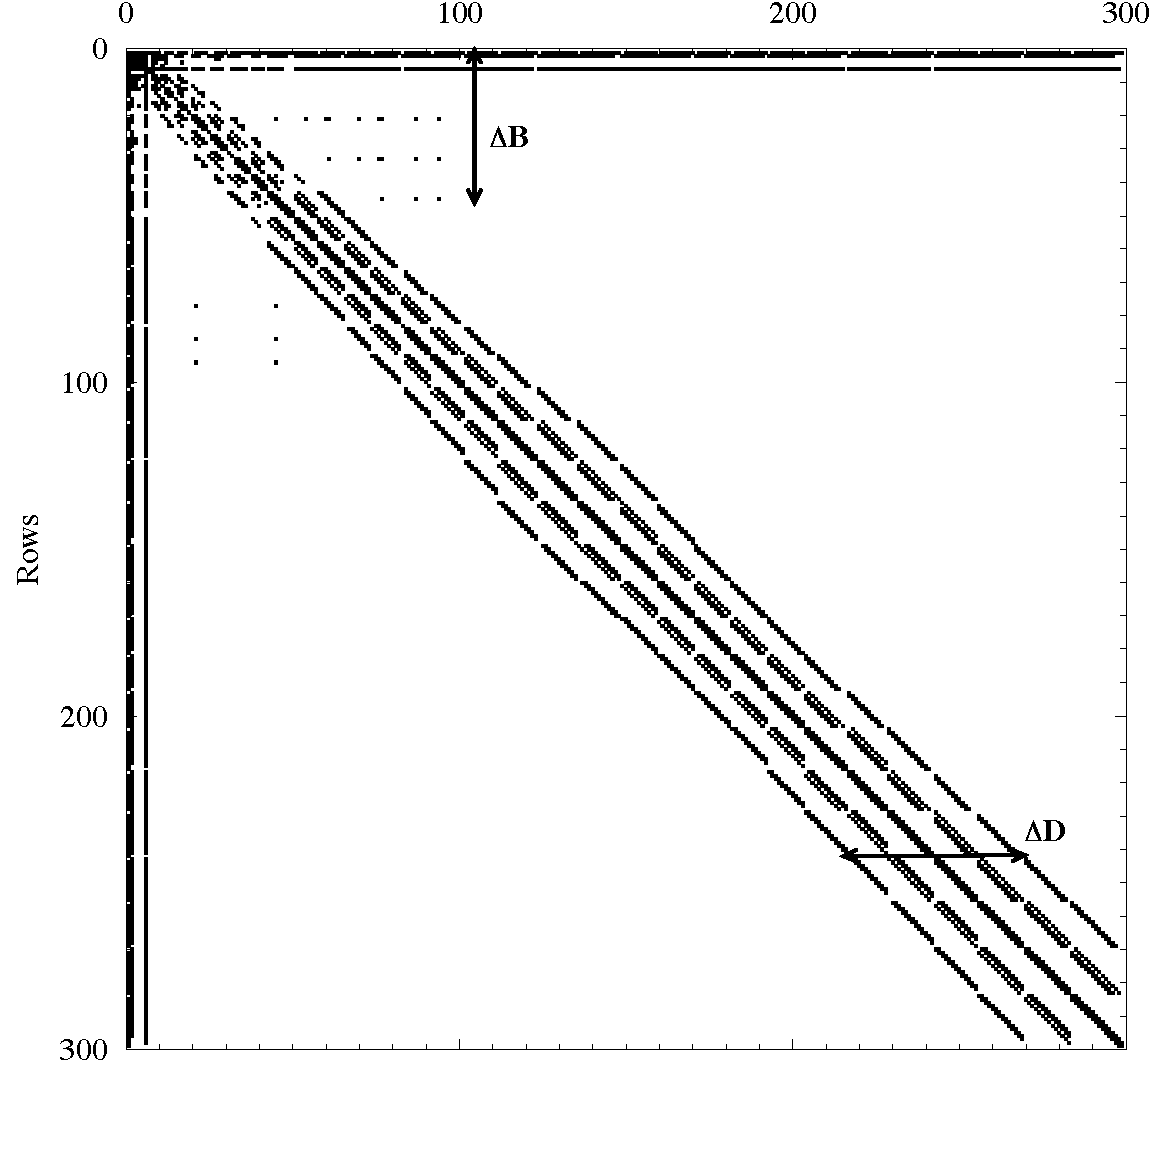
\includegraphics[width=.6\textwidth]{sparse}
    \end{center}
	\caption{Graphic demonstration of the sparseness of the Jacobian
	matrix.  The filled squares represent the non-zero elements.}
    \label{fig:sparse} 
\end{figure}

Fig.~\ref{fig:sparse} demonstrates the sparseness of the resulting Jacobian 
matrix, for a 300 nuclei network chosen to handle all the energy generating stages in the life of a massive star.  The nuclei are indexed in order of increasing Z and then A.  Of the 90,000 matrix elements, fewer than 5,000 are non-zero.  In terms of
the standard forms for sparse matrices, this Jacobian is best described
as doubly bordered, band diagonal.  With a border width, $\Delta B$, of
45 necessary to include the heavy ion reactions among \isotope{C}{12}, 
\isotope{O}{16} and \isotope{Ne}{20} along with the free neutrons, protons and
\alp -particles and a band diagonal width, $\Delta D$, of
54, even this sparse form includes almost 50,000 elements.  With solution
of the matrix equation consuming 90+\% of the computational time, there
is clearly a need for custom tailored solvers which take better advantage 
of the sparseness of the Jacobian \cite{PrAA87}. To date best results for small (N$<$100) matrices are obtained with machine optimized dense solvers (\eg\ LAPACK) or matrix specific solvers generated by symbolic processing \cite{Mull98,Mull86}.
For large matrices, generalized sparse solvers, both custom built and from
software libraries, are used (see, \cite{Timm99}).  

\bibliographystyle{apj}
\bibliography{apj_journals,add_journals,network,rspn_process,ccsn,sn-obs,stellar}

\end{document}